\documentclass[10pt, a4paper]{article}
\usepackage[top=3cm, bottom=4cm, left=3.5cm, right=3.5cm]{geometry}
\usepackage{sectsty} %设置章节标题的字体大小
\usepackage{amsmath,amsthm,amsfonts,amssymb,amscd, fancyhdr, color, comment, graphicx, environ}
\usepackage{float}
\usepackage{mathrsfs}
\usepackage[math-style=ISO]{unicode-math}
\setmathfont{Latin Modern Math}
\usepackage{lastpage}
\usepackage[dvipsnames]{xcolor}
\usepackage[framemethod=TikZ]{mdframed}
\usepackage{enumerate}
\usepackage[shortlabels]{enumitem}
\usepackage{fancyhdr}
\usepackage{indentfirst}
\usepackage{listings}
\usepackage{thmtools}
\usepackage{shadethm}
\usepackage{hyperref}
\usepackage{setspace}
\usepackage{anyfontsize} %字体大小
\usepackage{tcolorbox}
\usepackage{tikz}
\tcbuselibrary{theorems}


\hypersetup{
    colorlinks=true,
    linkcolor=blue,
    filecolor=magenta,      
    urlcolor=blue,
}
%%%%%%%%%%%%%%%%%%%%%%%%%%%%%%%%%%%%%%%%%%%%%%%%%%%%%%%%%%%%%%%%%%
%%%%%%%%%%%%%%%%%%%%%%%%%%%%%%%%%%%%%%%%%%%%%%%%%%%%%%%%%%%%%%%%%%
%Environment setup
\mdfsetup{skipabove=\topskip,skipbelow=\topskip}
\newrobustcmd\ExampleText{%
An \textit{inhomogeneous linear} differential equation has the form
\begin{align}
L[v ] = f,
\end{align}
where $L$ is a linear differential operator, $v$ is the dependent
variable, and $f$ is a given non-zero function of the independent
variables alone.
}
\mdfdefinestyle{theoremstyle}{%
linecolor=black,linewidth=1pt,%
frametitlerule=true,%
frametitlebackgroundcolor=gray!20,
innertopmargin=\topskip,
}
\mdtheorem[style=theoremstyle]{Problem}{Problem}
\newenvironment{Solution}{\textbf{Solution.}}

\definecolor{codegreen}{rgb}{0,0.6,0}
\definecolor{codegray}{rgb}{0.5,0.5,0.5}
\definecolor{codepurple}{rgb}{0.58,0,0.82}
\definecolor{backcolour}{rgb}{0.95,0.95,0.92}

\lstdefinestyle{mystyle}{
    backgroundcolor=\color{backcolour},   
    commentstyle=\color{codegreen},
    keywordstyle=\color{magenta},
    numberstyle=\tiny\color{codegray},
    stringstyle=\color{codepurple},
    basicstyle=\ttfamily\footnotesize,
    breakatwhitespace=false,         
    breaklines=true,                 
    captionpos=b,                    
    keepspaces=true,                 
    numbers=left,                    
    numbersep=5pt,                  
    showspaces=false,                
    showstringspaces=false,
    showtabs=false,                  
    tabsize=2
}

\lstset{style=mystyle}  %设置代码环境

%Page setup
\pagestyle{fancy}
\headheight 35pt
\lhead{\today}
\rhead{
\includegraphics[width=2.5cm]{logo-nju.jpg}}
\lfoot{}
\pagenumbering{arabic}
\cfoot{\small\thepage}
\rfoot{}
\headsep 1.2em
\renewcommand{\baselinestretch}{1.25}
%%%%%%%%%%%%%%%%%%%%%%%%%%%%%%%%%%%%%%%%%%%%%%%%%%%%%%%%%%%%%%%%%%
%%%%%%%%%%%%%%%%%%%%%%%%%%%%%%%%%%%%%%%%%%%%%%%%%%%%%%%%%%%%%%%%%%
%Add new commands here
\renewcommand{\labelenumi}{\alph{enumi})}
\newcommand{\Z}{\mathbb Z}
\newcommand{\R}{\mathbb R}
\newcommand{\Q}{\mathbb Q}
\newcommand{\NN}{\mathbb N}
\newcommand{\PP}{\mathbb P}
\DeclareMathOperator{\Mod}{Mod} 
\renewcommand\lstlistingname{Algorithm}
\renewcommand\lstlistlistingname{Algorithms}
\def\lstlistingautorefname{Alg.}
\newtheorem{theorem}{Theorem}
\newtheorem{lemma}{Lemma}
\newtheorem{case}{Case}
\newtheorem{definition}{Definition}
\newtheorem{example}{Example}
\renewcommand\proofname{Proof}
\newcommand{\assign}{:=}
\newcommand{\infixiff}{\text{ iff }}
\newcommand{\nobracket}{}
\newcommand{\backassign}{=:}
\newcommand{\tmmathbf}[1]{\ensuremath{\boldsymbol{#1}}}
\newcommand{\tmop}[1]{\ensuremath{\operatorname{#1}}}
\newcommand{\tmtextbf}[1]{\text{{\bfseries{#1}}}}
\newcommand{\tmtextit}[1]{\text{{\itshape{#1}}}}


%%%%%%%%%%%%%%%%%%%%%%%%%%%%%%%%%%%%%%%%%%%%%%%%%%%%%%%%%%%%%%%%%%
%%%%%%%%%%%%%%%%%%%%%%%%%%%%%%%%%%%%%%%%%%%%%%%%%%%%%%%%%%%%%%%%%%
%Begin now!




\begin{document}
% --------------------------------------------------------------------
% Definitions (do not change this)
% --------------------------------------------------------------------
\newcommand{\HRule}[1]{\rule{\linewidth}{#1}} 	% Horizontal rule

\makeatletter							% Title
\def\printtitle{%						
    {\centering \@title\par}}
\makeatother									

\makeatletter							% Author
\def\printauthor{%					
    {\centering \large \@author}}				
\makeatother							

% --------------------------------------------------------------------
% Metadata (Change this)
% --------------------------------------------------------------------
\title{	\normalsize \textsc{Time is precious; waste it wisely.} 	% Subtitle
		 	\\[2.0cm]								% 2cm spacing
			\HRule{0.5pt} \\						% Upper rule
			\LARGE \textbf{18.01 Single Variable Calculus}	% Title
			\HRule{2pt} \\ [0.5cm]		% Lower rule + 0.5cm spacing
			\normalsize 2023.10.1			% Todays date
		}

\author{
    Yining Wang\\	
    Nanjing University\\	
    \texttt{wyn20010707@gmail.com} \\
}

% ------------------------------------------------------------------------------
% Maketitle
% ------------------------------------------------------------------------------
\thispagestyle{empty}		% Remove page numbering on this page

\printtitle					% Print the title data as defined above
  	\vfill
%\begin{center}
%    
\includegraphics[width=0.4\textwidth]{logo-nju.jpg}\\
%\end{center}
\printauthor				% Print the author data as defined above
\newpage








\tableofcontents
\newpage

\section{Differentiation}
%%%%%%%%%%%%%%%%%%%%%%%%%%%%%%%%%%%%%%%%%%%%%%%%%%%%%%%%%%%%%%%%%%
%%%%%%%%%%%%%%%%%%%%%%%%%%%%%%%%%%%%%%%%%%%%%%%%%%%%%%%%%%%%%%%%%%
\subsection{Definition and Basic Rules}

\begin{definition}
    The derivative $f'(x_0)$ of $f$ at $x_0$ is the slope of the tangent line
    to $y = f(x)$ at the point $P = (x_0, f(x_0)$.
\end{definition}

Formula for the derivative:
\[
\hspace{2cm}
\begin{aligned}
    \underbrace{f'(x_0)}_{\text{derivative of } f \text{ at } x_0} &=
    \lim_{x \to 0} \frac{\Delta f}{\Delta x} &=
    \lim_{x \to 0} \underbrace{\frac{f(x_0+\Delta x)-f(x_0)}{\Delta x}}_{\text{difference quotient}}
\end{aligned}
\]

\begin{Problem}
    Does $f(x)=\left\lfloor x \right\rfloor $ have a derivative? If so, what is it? If not, why not?
\end{Problem}
\begin{Solution}
    The ``limit as $\Delta x$ approaches 0''  isn't
    well defined, so $f(x)$ is not differentiable at $x = 0$.
    (The left-hand limit and right hand limit are not equal)
\end{Solution}


\subsubsection*{Notations}
Just as there are many ways to express the same thing,
there are many notations for the derivative.
\begin{enumerate}
    \item $\Delta y = \Delta f$
    \item Taking the limit as $\Delta x \to 0$, we get
    \begin{enumerate}
        \item $\frac{\Delta y}{\Delta x} \to \frac{\mathrm{d}y}{\mathrm{d}x}$ (Leibniz' notation)
        \item $\frac{\Delta f}{\Delta x} \to f'(x_0)$ (Newton's notation)
    \end{enumerate}
\end{enumerate}

\begin{example}
    Find the derivative of $f(x)=x^n$ where $n=1,2,3\dots$ \\
    Here we have:
    \[
        \frac{\Delta y}{\Delta x}=\frac{(x+\Delta x)^n-x^n}{\Delta x}
    \]
    The \textbf{binomial theorem} tells us that:
    \[
        x^n+n(\Delta x)x^{n-1}+O\left((\Delta x)^2\right)
    \]
    where $O(\Delta x)^2$ is shorthand for 
    ``all of the terms with $(\Delta x)^2$,$(\Delta x)^3$
    ,and so on up to $(\Delta x)^n$''

    Now we have:
    \[
    \begin{aligned}
        \frac{\Delta y}{\Delta x}=\frac{(x+\Delta x)^n-x^n}{\Delta x}=\frac{(x^n+n(\Delta x)(x^{n-1})+O(\Delta x)^2)-x^n}{\Delta x}=nx^{n-1}+O(\Delta x)
    \end{aligned}
    \]
    and therefore,
    \[
        \frac{d}{dx}x^n = nx^{n-1}
    \]
\end{example}

Since we think about $\frac{\Delta y}{\Delta x}$ as the average change in $y$ over an interval of size $\Delta x$
The derivatives $\frac{dy}{dx}$ can also be taken as the instantaneous rate of change.


\begin{definition}
    The \textbf{right(left)-hand limit} of a function \(f(x)\) as \(x\) approaches \(a\)
    ,denoted as \(\lim_{{x \to a^+}} f(x)\), represents the value that \(f(x)\) approaches 
    as \(x\) gets arbitrarily close to \(a\) from the right (left) side 
    (i.e., from values greater than \(a\)).
\end{definition}

\begin{definition}
    A function $f$ is \textbf{continuous} at $x_0$ if \(\lim_{{x \to x_0}} f(x) = f(x_0)\). Which means:
    \begin{itemize}[label=$\ast$]  
        \item $\lim_{x\to x_0^+}f(x)=\lim_{x\to x_0^-}f(x)$; both of these one sided limits exist.
        \item $f(x_0)$ is defined.
        \item $\lim_{x\to x_0^+}f(x)=\lim_{x\to x_0^-}f(x)=f(x_0).$
    \end{itemize}

\end{definition}

\begin{definition}
    Discontinuity
    \begin{enumerate}
        \item A \textbf{jump discontinuity} occurs when the right-hand and left-hand limits exist but are not equal.
        \item At a \textbf{removable discontinuity}, the left-hand and right-hand limits are equal but
        either the function is not defined or not equal to these limits:
        \[
            \lim_{x\to x_0^+}f(x)=\lim_{x\to x_0^-}f(x)\neq f(x_0)    
        \]
        \item In an \textbf{infinite discontinuity}, the left- and right-hand limits are infinite.(e.g hyperbola)
    \end{enumerate}
\end{definition}

\begin{theorem}
    If $f$ is differentiable at $x_0$, then f is continuous at $x_0$.
\end{theorem}
\begin{proof}
    To show that:
    \[
        \lim_{x\to x_0}f(x) - f(x_0) = 0    
    \]
    \begin{align*}
        \lim_{x\to x_0}f(x) - f(x_0) &= \lim_{x\to x_0}\frac{f(x)-f(x_0)}{x-x_0}(x-x_0)\\
        &= f'(x_0)\cdot 0\\
        &= 0
    \end{align*}
    (we used the assumption that $f$ was differentiable when we wrote down $f'(x)$.)
\end{proof}

\subsubsection*{Derivative of $\sin x$ and $\cos x$, Algebraic Proof}
Begin with the definition of the derivative:
\[
    \frac{d}{dx}\sin x=\lim_{\Delta x\to0}\frac{\sin(x+\Delta x)-\sin(x)}{\Delta x}
\]
By using $\sin(a+b)=\sin(a)\cos(b)+\sin(b)\cos(a)$ we can get:
\[
\begin{aligned}
    \frac{d}{dx}\sin x &=\lim_{\Delta x\to0}\frac{\sin x\cos\Delta x+\cos x\sin\Delta x-\sin(x)}{\Delta x}\\
    &= \lim_{\Delta x\to0}\sin x\left(\frac{\cos\Delta x-1}{\Delta x}\right)+\lim_{\Delta x\to0}\cos x\left(\frac{\sin\Delta x}{\Delta x}\right)\\
\end{aligned}
\]
Here we introduce two important facts: \textbf{a)$\lim_{x\to 0}\frac{\sin x}{x} = 1$ b)$\lim_{x\to 0}\frac{\cos x -1}{x}$}.
Hence, we conclude:
\[
    \frac{d}{dx}\sin x = \cos x
\]
The calculation of the derivative of $\cos x$ is similar to that of the derivative of $\sin x$. 
The proof of the two properties above are ommitted here.

\begin{theorem}
    \textbf{Product Rule}
    \[
        (uv)' = u'v + uv'
    \]
\end{theorem}

\begin{proof}
    \begin{align*}
        (uv)' &= \lim_{\Delta x\to0}\frac{(uv)(x+\Delta x)-(uv)(x)}{\Delta x}  \\
        &= \lim_{\Delta x\to0}\frac{u(x+\Delta x)v(x+\Delta x)-u(x)v(x)}{\Delta x} \\
        &= \lim\limits_{\Delta x\to0}\frac{u(x+\Delta x)v(x)-u(x)v(x)+u(x+\Delta x)v(x+\Delta x)-u(x+\Delta x)v(x)}{\Delta x} \\
        &= \lim\limits_{\Delta x\to0}\left[\left(\frac{u(x+\Delta x)-u(x)}{\Delta x}\right)v(x)+u(x+\Delta x)\left(\frac{v(x+\Delta x)-v(x)}{\Delta x}\right)\right] \\
        &=u'(x)v(x)+u(x)v'(x)
    \end{align*}
\end{proof}

\begin{theorem}
    \textbf{Quotient Rule}
    \[
        \left(\frac uv\right)'=\frac{u'v-uv'}{v^2}
    \]
\end{theorem}

\begin{theorem}
    \textbf{Chain Rule}:The derivative of a composition of functions is a product. 
    \[
        \lim_{\Delta t\to0}\frac{\Delta y}{\Delta t}=\frac{dy}{dt}=\frac{dy}{dx}\frac{dx}{dt}
    \]
\end{theorem}

\subsubsection*{Notations}
Higher derivatives are derivatives of derivatives.
\[
    \begin{array}{|c|c|c|c|}
        \hline
        f'(x) & Df & \frac{df}{dx} & \frac{d}{dx}f \\
        f''(x) & D^2 f & \frac{d^2f}{dx^2} & \left(\frac{d}{dx}\right)^2f \\
        f'''(x) & D^3 f & \frac{d^3f}{dx^3} & \left(\frac{d}{dx}\right)^3f \\
        f^{(n)}(x) & D^n f & \frac{d^nf}{dx^n} & \left(\frac{d}{dx}\right)^nf \\
        \hline
    \end{array}
\]
The symbol $\frac{d}{dx}$ represent “operators” which can be applied to a function. 
This explains why the two powers are in different locations.

\subsection{Implicit Differentiation and Inverse Functions}
%%%%%%%%%%%%%%%%%%%%%%%%%%%%%%%%%%%%%%%%%%%%%%%%%%%%%%%%%%%%%%%%%%
%%%%%%%%%%%%%%%%%%%%%%%%%%%%%%%%%%%%%%%%%%%%%%%%%%%%%%%%%%%%%%%%%%
\subsubsection*{Implicit Differentiation (Rational Exponent Rule)}
\[
    (x^a)' = ax^{a-1}, \forall x \in \mathbb{Q} 
\]

\begin{example}
    \textbf{Slope of a line tangent to a circle - Direct version} \\
    The graph of $x^2 + y^2 = 1$ is a circle of ridius 1 centered at the origin. 
    This equation can't be written in a form of $y = f(x)$ since every $x$ has two corresponding $y$ values.
    \[
        x^2 + y^2 = 1
    \]
    \[
        y = \pm \sqrt{1 - x^2}
    \]
    Now we just focus on the top half of the unit circle. By using the chain rule, we can have: 
    \[
        \frac{dy}{dx}=\frac12u^{-1/2}\cdot(-2x)=-x\cdot(1-x^2)^{-1/2}=\frac{-x}{\sqrt{1-x^2}}.
    \]
    \textbf{Slope of a line tangent to a circle - Implicit version} \\
    Instead of solving for $y$, we could just imply the operator $\frac{d}{dx}$ to both side of the original equation:
    \begin{align*}
        x^2 + y^2 &= 1 \\
        \frac{d}{dx} (x^2) + \frac{d}{dx} (y^2) &= 0 \\
        2x + 2y\frac{dy}{dx} &= 0 \\
        \frac{dy}{dx} &= -\frac{x}{y}
    \end{align*}
    We get the same answer and it works for both sides of the unit circle.
    Implicit differentiation simplified this calculation.
\end{example}
\begin{example}
    \textbf{Derivative of the Inverse of a Function}\\
    If $f(x) = y$ and $g(y) = x$, then $g$ is the inverse of $f$ ($g = f^{-1}$) and $f$ is the inverse of $g$.
    The graph of $f ^{-1}$ is the reflection of the graph of $f$ across the line $y = x$. So we have:
    \[
        \frac d{dy}(f^{-1}(y))=\frac1{\frac{dy}{dx}}.
    \]
    An example of this is the derivative of $y = \arctan(x)$. We can start from its inverse: $\tan y = x$
    \begin{align*}
        \tan y &= x \\
        \frac{d}{dx}\tan y &= \frac{d}{dx}x \\
        \left(\frac{1}{(\cos y)^2}\right)\frac{dy}{dx} &= 1 \\
        \frac{dy}{dx}\quad &= \quad\cos^2(y)\\
        \frac d{dx}\arctan(x)&=\frac1{1+x^2}. 
    \end{align*} 
\end{example}

\subsubsection*{Derivative of $a^x$}
\begin{proof}
    \begin{align*}
        a^x=\left(e^{\ln(a)}\right)^x &=e^{x\ln(a)} \\
        \frac d{dx}e^{(\ln a)x}\quad &=\quad(\ln a)e^{(\ln a)x} \\
        \frac d{dx}a^x &=(\ln a)a^x
    \end{align*}

\end{proof}

\begin{example}
    \textbf{Derivative of $x^x$}
    First, let $x$ denote $x^x$, then we take the natural log of both sides:
    \[\ln v = x\ln x\]
    Next, we differentiate both sides of the equation,:
    \begin{align*}
        (\ln v)' &= \ln x + x\cdot\frac{1}{x} \\
        \frac{v'}{v} &= \frac{1}{x} \\  
    \end{align*}
    Plugging in $x^x$ for $v$ and solving for $v'$, we get:
    \[\frac d{dx}x^x\quad=\quad x^x(1+\ln x)\]
\end{example}
    
\section{Applications of Differentiation}
%%%%%%%%%%%%%%%%%%%%%%%%%%%%%%%%%%%%%%%%%%%%%%%%%%%%%%%%%%%%%%%%%%
%%%%%%%%%%%%%%%%%%%%%%%%%%%%%%%%%%%%%%%%%%%%%%%%%%%%%%%%%%%%%%%%%%
\subsection{Approximation and Curve Sketching}
\subsubsection*{Linear Approximation}
\begin{example}
    \textbf{Linear Approximation to lnx at $x=1$} \\
    For a given curve \(y = f(x)\), it is approximately the same as its tangent line:
    \[ \boxed{y = f(x_0) + f'(x_0)(x - x_0)} \]
    
    Let $f(x) = lnx$. Then the formula for linear approximation tells us that:
    \begin{align*}
        f(x)& \approx\quad f(x_0)+f'(x_0)(x-x_0) \\
       \text{ln x} &\approx\quad\ln(1)+1(x-1)  \\
        \text{ln x} &\approx\quad0+(x-1)  \\
        \operatorname{ln}x &\approx\quad(x-1) 
    \end{align*}
    When x is close to the base point $x_0$, the point of linear approximation is that the curve is
    approximately the same as the tangent line.
\end{example}

\begin{example}
    \textbf{Approximations at 0 for Sine, Cosine and Exponential Functions}
    Based on the formula $f(x) \approx f(0) + f'(0)x $, we have:
    \begin{enumerate}
        \item $\sin x \approx x$ (if $x \approx 0$)
        \item $\cos x \approx 1$ (if $x \approx 0$)
        \item $e^x \approx 1 + x$ (if $x \approx 0$)
    \end{enumerate}
\end{example}

\begin{example}
    \textbf{Approximations at 0 for $ln(1 + x)$ and $(1 + x)^r$}\\
    1. $ln(1+x) \approx x$ (if $x \approx 0$)\\
    2. $(1+x)^r \approx 1 + rx $ (if $x \approx 0$)
\end{example}

\subsubsection*{Quadratic Approximation}
Quadratic approximation is an extension of linear approximation by adding one more term:
\[ \boxed{f(x)\approx\underbrace{f(x_0)+f'(x_0)(x-x_0)}_\text{Linear Part}+\underbrace{\frac{f''(x_0)}2(x-x_0)^2}_\text{Quadratic Part}\quad(x\approx x_0)} \]
According to the equation above, we can calculate the following approximations:
\begin{itemize}
    \item $\sin x\approx x$  \quad(if $x \approx 0$)
    \item $\cos x\approx1-\frac{x^2}2$  \quad(if $x \approx 0$)
    \item $e^x\approx1+x+\frac12x^2$  \quad(if $x \approx 0$)
    \item $\ln(1+x)\approx x-\frac12x^2$  \quad(if $x \approx 0$)
    \item $(1+x)^r\approx 1+rx+\frac{r(r-1)}{2}x^2$  \quad(if $x \approx 0$)
\end{itemize}

\begin{Problem}
    The linear approximation of $\frac{e^{-3x}}{\sqrt{1+x}}=e^{-3x}(1+x)^{-1/2}.$
\end{Problem}
\begin{Solution}
    \[e^{-3x}(1+x)^{-1/2}\approx\left(1+(-3x)+\frac12(-3x)^2\right)\left(1+\left(-\frac12\right)x+\frac{\left(-\frac12\right)\left(-\frac32\right)}2x^2\right)\]
    \[e^{-3x}(1+x)^{-1/2}\approx1-\frac{7}{2}x+\frac{51}{8}x^2\]
\end{Solution}

\begin{definition}
    If $f'(x_0) = 0$, we call $x_0$ a critical point and $y_0 = f(x_0)$ is a critical value of f.
\end{definition}

\subsubsection*{General Strategy for Graph Sketching}
\begin{enumerate}
    \item \textbf{Special points:} discontinuities of \(f\), end points, easy points\dots 
    \item \textbf{Check \(f'(x)\):} critical points 
    \item \textbf{Check \(f''(x)\):} concave up or down?
\end{enumerate}

\subsection{Optimization, Related Rates and Newton's Method}
\begin{Problem}
    Find the box (without a top) with least surface area for a fixed volume.[square bottom]
\end{Problem}
\begin{Solution}
    \textbf{[Direct Solution]}
    Let x denote width and length, y denote height. We have the
    \textit{constraint} that the box must have a certain volume:
    \[y = \frac{V}{x^2}\]
    The surface of the box can be written as:
    \[A(x)\quad=\quad x^2+\frac{4V}x\]
    To find the critical points we take the derivative of $A(x)$ and set it equal to zero.
    \begin{align*}
        A^{\prime}(x)\quad &= \quad2x-\frac{4V}{x^2} = 0 \\
        x &= (2V)^{\frac{1}{3}}
    \end{align*}
    Then we can check end points and obtain the final answer (Here we use dimensionless variables):
    \[\frac{x}{y} = 2\]
    \textbf{[Implicit Solution]}
    \[\frac d{dx}V=2xy+x^2\frac{dy}{dx}\Longrightarrow0=2xy+x^2y^{\prime}\]
\end{Solution}

\begin{Problem}
    \textbf{Related Rates, A Conical Tank} \\
    Consider a conical tank whose radius at the top is 4 feet and whose
    depth is 10 feet. It's being filled with water at the rate of 2 cubic feet per
    minute. How fast is the water level rising when it is at depth 5 feet?
\end{Problem}

\begin{Solution}
    The volume of a cone is $\frac13\pi r^2h$. We have: 
    \[V=\frac13\cdot\underbrace{\pi r^2}_{\mathrm{base}}\cdot\underbrace{h}_{\mathrm{height}}\]\
    We can use the Chain Rule to find the rate of change of height with respect to time:
    \begin{align*}
        \frac{dV}{dt}& \begin{aligned}=\quad\frac{dV}{dh}\frac{dh}{dt}\end{aligned}  \\
        &=\quad\frac\pi3\left(\frac25\right)^23h^2\frac{dh}{dt} \\
        &=\quad\frac4{25}\pi h^2h^{\prime}
    \end{align*}
    We know that $V' = 2$ and $h = 5$ when we want to find $h^{\prime}$, so we can plug these values in:
    \begin{align*}
        2&=\quad\frac4{25}\pi\cdot5^2\cdot h^{\prime} \\
        h^{\prime}&=\quad\frac{1}{2\pi} 
    \end{align*}
\end{Solution}

\begin{theorem}
    \textbf{Newton's Method} \\
    Newton's method is a way to approximate the roots of a function. 
    It is based on the idea that if $x$ is close to a root of $f$, then $f(x)$ is close to 0. 
    So we can approximate the root by finding the $x$-intercept of the tangent line to the graph of $f$ at $(x, f(x))$.
    \[x_{n+1}=x_n-\frac{f(x_n)}{f'(x_n)}\]
    The size of the error is proportional to the square of the size of the previous error. Newton's method works well if the initial guess is close to the root.
\end{theorem}

\subsection{Mean Value Theorem, Antiderivatives and Differential Equations}
\begin{theorem}
    \textbf{Mean Value Theorem} \\
    If $f$ is continuous on $[a, b]$ and differentiable on $(a, b)$, then there exists a point $c$ in $(a, b)$ such that:
    \[\boxed{f'(c)=\frac{f(b)-f(a)}{b-a}}\]
\end{theorem}

\subsubsection*{The Mean Value Theorem and Linear Approximation}
The linear approximation of $f$ at $x = a$ has the formula:
\[f(x)\approx f(a)+f'(a)(x-a)\]
If we let $\Delta x = x - a$, then we can rewrite this as:
\[\frac{\Delta Y}{\Delta X} \approx f'(a)\]
Similarly, the Mean Value Theorem says that:
\[\exists c \in (a, b) \quad s.t. \quad f(b) = f(a) + f'(c)(b - a)\]
which can be rewritten as:
\[\exists c \in (a, b) \quad s.t. \quad \frac{\Delta Y}{\Delta X} = f'(c)\]
The average change in $y$ over an interval is between the maximum and minimum values of $f'(x)$. 
During a trip, the average speed of a car is between the maximum and minimum speeds:
\[\min_{a\leq x\leq b}f'(x)\leq\frac{f(b)-f(a)}{b-a}=f'(c)\leq\max_{a\leq x\leq b}f'(x)\]

\begin{definition}
    \textbf{Differential} \\
    The differential of a function $y = f(x)$ is defined as:
    \[dy = f'(x)dx\]
\end{definition}
\ast  Recall the relation between differentials and linear approximation

\begin{definition}
    \textbf{Antiderivative} \\
    $G(x) = \int g(x)dx$ is an antiderivative of $g(x)$. Other ways of writing antiderivatives are:
    \[G'(x) = g(x)\quad\text{or}\quad dG = g(x)dx\]
\end{definition}

\begin{example}
    \textbf{Antiderivative of $\frac{1}{x}$}
    \begin{align*}
        \int\frac{1}{x}dx &= \int x^{-1}dx \\
        &= \ln|x| + c
    \end{align*}
\end{example}

\subsubsection*{Antiderivatives are Unique up to a Constanttitle}
\begin{theorem}
    If $F'(x) = f(x)$ and $G'(x) = f(x)$, then \boxed{$F(x) = G(x) + c$} for some constant $c$.
    \begin{proof}
        If $F'(x) = G'(x)$, then $(F - G)'(x) = 0$. By the \textbf{Mean Value Theorem}, $\exists c$ such that
        $G(x) - F(x) = c$. So $G(x) = F(x) + c$.
    \end{proof}  
\end{theorem}

"This is a very important fact. It's the basis for calculus; the reason why it makes sense to do calculus at all."

\subsubsection*{Introduction to Ordinary Differential Equations}
\begin{example}
    \textbf{$\frac{dy}{dx} + xy  = 0$} \\
    The first step to solve it is to separate $\frac{dy}{dx}$:
    \[\frac{dy}{y} = -xdx\]
    Then we integrate both sides:
    \[\int\frac{dy}{y} = \int-xdx\]\
    \[\ln y = -\frac{x^2}{2} + c \quad\text{assume } y > 0\]
    \[ y\quad=\quad Ae^{-x^2/2}\quad(A=e^c) \]
    This function is known as the normal distribution.
\end{example}

\section{The Definite Integral and its Applications}
\subsection{Definition of the Definite Integral and First Fundamental Theorem}
\begin{definition}
    \textbf{Riemann Sum} \\
    Let $f$ be a function defined on $[a, b]$. The general procedure for computing the definite integral 
    $\int_a^bf(x)dx$ is to approximate the area under the curve $y = f(x)$ by the sum of the areas of rectangles:
    \[S_n = \sum_{i=1}^nf(x_i^*)\Delta x\]
    where $\Delta x = \frac{b - a}{n}$ and $x_i^*$ is any point in the $i$th subinterval $[x_{i-1}, x_i]$.\\
    In the limit as n goes to infinity, this sum approaches the value of the definite integral:
    \[\lim_{n\to\infty}S_n = \int_a^bf(x)dx\]
\end{definition}

\subsubsection*{The Fundamental Theorem of Calculus}
\begin{theorem}
    \textbf{First Fundamental Theorem of Calculus} \\
    If $f$ is continuous on $[a, b]$ and $F'(x) = f(x)$ for all $x$ in $[a, b]$, then:
    \[\boxed{\int_a^bf(x)dx = F(b) - F(a) = F(x) \Big|_a^b}\]
\end{theorem}

\begin{proof}
    We can define $G(x) = \int_a^x f(t)dt$. Then $G'(x) = f(x)$ by the \textbf{Second Fundamental Theorem of Calculus}.
    Since $F'(x) = G'(x)$, we have $F(x) = G(x) + c$ for some constant $c$.
    \begin{align*}
        F(b)-F(a) &= G(b)+c-(G(a)+c) \\
        &= G(b)-G(a) \\
        &= \int_a^b f(t)dt
    \end{align*}  
\end{proof}

\begin{Problem}
    \textbf{Area under one “hump” of sin(x).}
\end{Problem}
\begin{Solution}
    \begin{align*}
        \int_0^{\pi}\sin xdx &= -\cos x\Big|_0^{\pi} \\
        &= -\cos\pi + \cos0 \\
        &= 2
    \end{align*}
\end{Solution}

\subsubsection*{An Interpretation of the Fundamental Theorem of Calculus}
\textbf{Speed and distance are very helpful in understanding the definite integral!!! } \\
Let t denote time, $v(t)$ denote velocity, and $s(t)$ denote distance. Then:
\[\int_a^b v(t)dt = s(b) - s(a)\] 
It's very reasonable to think that the distance traveled is the area under the velocity curve.
\[\sum_{i=1}^nv(t_i)\Delta t\approx\int_a^bv(t)dt\]
The Riemann sum, on the left, is approximately how far the object travels, and the definite integral, on the right, is the exact distance traveled.

\subsubsection*{Properties of Integrals}
\begin{enumerate}
    \item \[ \int_a^b[f(x) + g(x)]dx = \int_a^bf(x)dx + \int_a^bg(x)dx\]
    \item \[ \int_a^b cf(x)dx = c\int_a^bf(x)dx \]
    \item \[ \int_a^b f(x)dx + \int_b^c f(x)dx = \int_a^c f(x)dx \]
    \item \[ \int_a^a f(x)dx = 0\]
    \item \[ \int_a^b f(x)dx = -\int_b^a f(x)dx \]
    \item (Estimation) If $f(x) \leq g(x)$ and $a < b$, then:
    \[ \int_a^b f(x)dx \leq \int_a^b g(x)dx \]
    \item (Change of Variables or “Substitution”) If $u = u(x) $ then $du = u'(x)$ and $\int g(u)du = \int g(u(x))u'(x)dx$.
    \[ \int_{u_1}^{u_2}g(u)du=\int_{x_1}^{x_2}g(u(x))u^{\prime}(x)dx \]
    where $u'$ does not change sign. (If it does, we need to split the integral into pieces.)
\end{enumerate}

\subsubsection*{The Fundamental Theorem and the Mean Value Theorem}
The \textbf{first fundamental theorem} can be weitten as:
\[\Delta F = \int_a^b f(x)dx\]
If we divide both sides by $\Delta x$, we get:
\[\frac{\Delta F}{\Delta x} = \underbrace{\frac{1}{b-a}\int_a^b f(x)dx} _{\text{average value of } f(x)}\]
We can rewrite \textbf{FTC1} as:
\[\Delta F = Average(F')\Delta x \]
And we rewrite \textbf{MVT} as:
\[\Delta F = F'(c)\Delta x \quad \text{(Here $c$ is not specific) }\]
Even if we don't know exactly what $c$ is, we can still get:
\[\left(\min_{a<x<b}F'(x)\right)\Delta x\leq\Delta F=F'(c)\Delta x\leq\left(\max_{a<x<b}F'(x)\right)\Delta x.\]
The \textbf{FTC1} gives us a little more information:
\[\left(\min_{a<x<b}F'(x)\right)\Delta x\leq\Delta F=\text{Average}F'\Delta x\leq\left(\max_{a<x<b}F'(x)\right)\Delta x.\]

\begin{Problem}
    \textbf{The Mean Value Theorem and Estimation} \\
    Given that $F'(x)  = \frac{1}{x+1}$ and $F(0) = 1$, the mean value theorem implies that $A < F(4) < B$ for which $A$ and $B$?
\end{Problem}
1. \textbf{MVT}:
\[F(4) - F(0) = F'(c)(4 - 0)\]
\[\frac{1}{5} < \frac{F(4) - F(0)}{4} < 1\]
\[\frac{9}{5} < F(4) < 5\]
2. \textbf{FTC1}:
Based on the \textbf{FTC1}, we can get:
\[F(4) - F(0) = \int_0^4 \frac{1}{x+1}dx\]
Based on the graph of $\frac{1}{x+1}$, we can get:
\[F(4)-F(0)=\int_0^4\frac{dx}{1+x}<\int_0^41dx=4 \text{ and } F(4) - F(0) = \int_0^4 \frac{dx}{1+x} > \int_0^4\frac{1}{5}dx = \frac{4}{5}\]
Again we can get:
\[\frac{9}{5}\text{(lower Riemann sum)} < F(4) < 5\text{(upper Riemann sum)}\]

\subsection{Second Fundamental Theorem, Areas, Volumes}
\begin{theorem}
    \textbf{Second Fundamental Theorem of Calculus} \\
    If $f$ is continuous and $ G(x) = \int_a^x f(t)dt$, then 
    \[\boxed{G'(x) = f(x)}\]
    G(x) solves the differential equation $G'(x) = f(x)$ and $G(a) = 0$.
\end{theorem}

\begin{proof}
    Since G(x) is the area under the curve $y = f(t)$ from $t = a$ to $t = x$, we can write:
    \[\Delta G \approx f(x)\Delta x\]
    then we can get $\frac{\Delta G}{\Delta x} \approx f(x)$, which means:
    \[G'(x) = \lim_{\Delta x\to0}\frac{\Delta G}{\Delta x} = f(x)\] 
\end{proof}    

\begin{example}
    \textbf{Log of a Product} \\
    L(x) is an alternatively defined logarithm function.Show that $L(ab) = L(a) + L(b)$.
    \begin{align*}
        L(ab) &= \int_1^{ab}\frac{1}{x}dx \\
        &= \int_1^a\frac{1}{x}dx + \int_a^{ab}\frac{1}{x}dx \\
        &= \int_1^a\frac{1}{x}dx + \int_1^b\frac{1}{u}du \quad (u = ax) \\
        &= L(a) + L(b)
    \end{align*}
\end{example}

\subsubsection*{Area between two curves}
\begin{center}
\begin{tikzpicture}
        % Define the functions
    \def\fOne{0.5 * \x^2}
    \def\fTwo{0.2 * \x^3}

    % Draw the curves
    \draw[domain=0:2, smooth, variable=\x, blue] plot ({\x}, {\fOne});
    \draw[domain=0:2, smooth, variable=\x, red] plot ({\x}, {\fTwo});

    % Fill the area between the curves
    \fill[gray!30] (0,0) -- plot[domain=0:2, smooth, variable=\x] ({\x}, {\fOne}) -- plot[domain=2:0, smooth, variable=\x] ({\x}, {\fTwo}) -- cycle;

    % Add labels and axes
    \draw[->] (-0.5,0) -- (3,0) node[right] {$x$};
    \draw[->] (0,-0.5) -- (0,3) node[above] {$y$};
    \node[blue] at (1.5,2.5) {$y = f(x)$};
    \node[red] at (1.5,0.8) {$y = g(x)$};
\end{tikzpicture}
\end{center}

 By using the idea of Riemann sum, we can get the area between two curves:
\[ A=\int_a^b\left(f(x)-g(x)\right)dx\]
\begin{example}
    \textbf{Find the area between $x = y^2$ and $y = x - 2$}\\
    Hard Way: Slice the region into vertical strips and integrate with respect to $y$.\\
    Easy Way: Slice the region into horizontal strips and integrate with respect to $x$.
\end{example}

\begin{example}
    \textbf{Volume of a Sphere}
    \begin{center}
        \begin{tikzpicture}
            % Draw the circle
            \draw (2,0) circle [radius=2];
        
            % Add labels and axes
            \draw[->] (-1,0) -- (5,0) node[right] {$x$};
            \draw[->] (0,-2.5) -- (0,2.5) node[above] {$y$};
            \node[fill=black, circle, inner sep=2pt, label={above right:$(a,0)$}] at (2,0) {};
        \end{tikzpicture}
    \end{center}
    \begin{align*}
        V &= \int_{0}^{2a} \pi y^2dx \\
        &= \pi\int_{0}^{2a} (a^2 - x^2)dx \\
        &= \pi\left(a^2x - \frac{x^3}{3}\right)\Big|_{0}^{2a} \\
        &= \frac{4}{3}\pi a^3
    \end{align*}
\end{example}

\subsection{Average Value, Probability and Numerical Integration}
\subsubsection*{Average Value of a Function}
\begin{definition}
    \textbf{Average Value of a Function} \\
    The average value of a function $f$ on the interval $[a, b]$ is:
    \[\boxed{f_{avg} = \frac{1}{b-a}\int_a^b f(x)dx}\]
\end{definition}

\begin{example}
    \textbf{Average Height of a unit semicircle (with respect to horizontal distance)} \\
    \begin{align*}
        Avg(f) &= \frac{1}{2}\int_{-1}^{1}\sqrt{1-x^2}dx \\
        &= \frac{1}{2}\text{Area of a unit semicircle} \\
        &= \frac{\pi}{4}
    \end{align*}

    \textbf{Average with Respect to Arc length} \\    
    \begin{align*}
        Avg(f) &= \frac{1}{\pi}\int_{0}^{\pi}\sin \theta d\theta \\
        &= \frac{1}{\pi}\left(-\cos \theta\right)\Big|_{0}^{\pi} \\
        &= \frac{2}{\pi}
    \end{align*} 
\end{example}

\subsubsection*{Weighted Average}
\[\frac{\int_a^bf(x)w(x)dx}{\int_a^bw(x)dx}\]

\begin{example}
    \textbf{Boy Near a Dart Board}\label{boy-dartboard}\\
    (cf. \href{https://ocw.mit.edu/courses/18-01sc-single-variable-calculus-fall-2010/resources/mit18_01scf10_ses62d/}{OCW})
\end{example}

\subsubsection*{Numerical Integration}
\begin{enumerate}
    \item \textbf{Riemann Sums}
    \item \textbf{Trapezoidal Rule}
        % use a graph to show the trapezoidal rule
        \begin{center}
            \begin{tikzpicture}
                % Draw the curve using plot and coordinates
                \draw[blue, thick, domain=1:4] plot[smooth] coordinates {(1,0.84) (2,1.84) (3,0.84) (4,0.5)};
            
                % Draw the trapezoids
                \draw[fill=gray!30] (1,0) -- (1,0.84) -- (2,1.84) -- (2,0) -- cycle;
                \draw[fill=gray!30] (2,0) -- (2,1.84) -- (3,0.84) -- (3,0) -- cycle;
                \draw[fill=gray!30] (3,0) -- (3,0.84) -- (4,0.5) -- (4,0) -- cycle;
            
                % Draw the x-axis
                \draw[->] (-0.5,0) -- (5,0) node[right] {$x$};
                % Draw the y-axis
                \draw[->] (0,-0.5) -- (0,2) node[above] {$y$};
            
                % Add labels
                \node at (1,-0.2) {$a$};
                \node at (4,-0.2) {$b$};
                \node at (1,0.84+0.5 ) {$f(a)$};
                \node at (2,1.84+0.2) {$f(x_1)$};
                \node at (2,-0.2) {$x_1$};
                \node at (3,0.84+0.2) {$f(x_2)$};
                \node at (3,-0.2) {$x_2$};
                \node at (4,0.5+0.2) {$f(b)$};
            \end{tikzpicture}
        \end{center}
        \[Area = \Delta x\left\{\frac{y_o+y_1}2+\frac{y_1+y_2}2+\frac{y_2+y_3}2+...+\frac{y_{n-1}+y_n}2\right\}\]
        Notice that it's the average of the left and right Riemann sums.
    \item \textbf{Simpson's Rule}
        the essence of Simpson's rule is to approximate the function by a quadratic polynomial.
\end{enumerate}

\subsubsection*{Area Under the Bell Curve}
In the example \ref{boy-dartboard}, we get the volume of revolution of the bell curve:
\begin{align*}
    V &= \int_0^\infty2\pi r\mathrm{~}e^{-r^2}dr\\
    &= -\pi e^{-r^2}\Big|_0^\infty\\
    &= \pi
\end{align*}
Then we let Q denote the area under the bell curve:
\[ Q = \int_{-\infty}^\infty e^{-t^2}dt \]
To calculate Q, we need to use a trick that we don't know yet:
\[\boxed{Q^2  = V}\]
\begin{figure*}
    \centering
    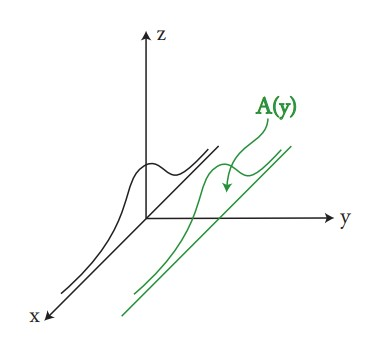
\includegraphics[width=0.3\textwidth]{Slices.jpg}
    \caption{Three-dimensional slices of the volume of rotation of $e^{-r^2}$.}
\end{figure*}
\begin{figure*}
    \centering
    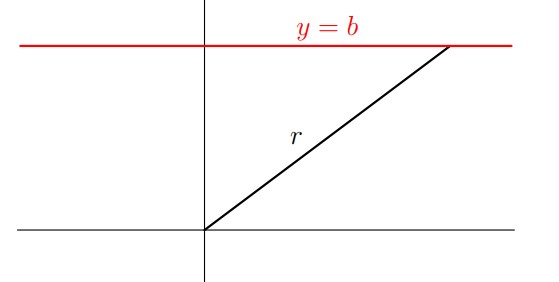
\includegraphics[width=0.3\textwidth]{topview.jpg}
    \caption{Top view of a slice of the surface of revolution of $e^{-r^2}$.}
\end{figure*}

The formula for volume by slices is:
\[ V = \int_-\infty^\infty A(y)dy \]
then we fix $y= b$ and calculate $A(b)$. From the figure above, we can get: $b^2 + x^2 = r^2$. 
The height of the surface at a point r units away from (0, 0) is given by: 
\begin{align*}
    height &= e^{-r^2} \\
    &= e^{-(b^2 + x^2)} \\
\end{align*}
The area of the slice is:
\begin{align*}
    A(b) &= \int_{-b}^b e^{-(b^2 + x^2)}dx \\
    &= e^{-b^2}\int_{-b}^b e^{-x^2}dx \\
    &= e^{-b^2}Q
\end{align*}
Finally, we can get:

\begin{align*}
    V & =\quad\int_{-\infty}^{\infty}A(y)dy  \\
    &=-\int_{-\infty}^{\infty}e^{-y^2}Qdy \\
    &= Q\int_{-\infty}^{\infty}e^{-y^2}dy \quad\text{($Q$ is a constant)} \\
    &= Q^2 \quad\text{(by definition, } Q=\int_{-\infty}^\infty e^{-t^2}dt).
\end{align*}

\section{Techniques of Integration}
\subsection{Trigonometric Powers, Trigonometric Substitution and Completing the Square}
\begin{example}
    \textbf{Integrating $\int \sin ^3 x dx$} \\
    We can use the identity $\sin ^2 x = 1 - \cos ^2 x$ to rewrite the integral as:
    \begin{align*}
        \int \sin ^3 x dx &= \int \sin x (1 - \cos ^2 x)dx \\
        &= \int \sin x dx - \int \sin x \cos ^2 x dx \\
        &= -\cos x - \int \sin x \cos ^2 x dx
    \end{align*}
    Then we can use the substitution $u = \cos x$ to solve the second integral:
    \begin{align*}
        \int \sin x \cos ^2 x dx &= \int -u^2 du \\
        &= -\frac{u^3}{3} + C \\
        &= -\frac{\cos ^3 x}{3} + C
    \end{align*}
    Finally, we can get:
    \[\int \sin ^3 x dx = -\cos x + \frac{\cos ^3 x}{3} + C\]
\end{example}

\subsubsection*{Trig Substitution}
\begin{center}
    \begin{tabular}{|c|c|c|}
        \hline
        If your integrand contains: & Make substitutions: & So that: \\
        \hline
        $\sqrt{a^2-x^2}$ & $x = a\sin\theta$ & $dx = a\cos\theta d\theta$ \\
    
        $\sqrt{a^2+x^2}$ & $x = a\tan\theta$ & $dx = a\sec^2\theta d\theta$ \\
    
        $\sqrt{x^2-a^2}$ & $x = a\sec\theta$ & $dx = a\sec\theta\tan\theta d\theta$ \\
        \hline
    \end{tabular}
\end{center}

\subsection{Partial Fractions, Integration by Parts, Arc Length, and Surface Area}

\subsubsection*{Introduction to the Cover-up Method}
Take an integral for example:
\[\int \frac{4x -1}{x^2 + x - 2}dx\]
\begin{enumerate}
    \item First we factor the denominator: $x^2 + x - 2 = (x + 2)(x - 1)$:
    \item Next we write the fraction as a sum of two fractions:
    \[\frac{4x -1}{x^2 + x - 2} = \frac{A}{x - 1} + \frac{B}{x + 2}\]
    \item We solve for $A$ by multiplying both sides by $x - 1$:
    \[ \frac{4x-1}{x+2} = A + \frac{B(x-1)}{x+2} \]
    then we plug in $x = 1$ to get $A$:
    \[\frac{4 - 1}{1 + 2} = A + 0 \Longrightarrow A = 1\]
    By applying the same method, we can get $B = 3$.
\end{enumerate}

\subsubsection*{Repeated Factors}
\begin{example}
    \textbf{$\frac{x^2 + 2}{(x-1)^2 (x+2)}$}\\
    In general, when there is a repeated factor in the denominator, we need to add a term for each power of the factor up to the power of the factor in the denominator:
    \[
        \frac{x^2 + 2}{(x-1)^2 (x+2)} = \frac{A}{x-1} + \frac{B}{(x-1)^2} + \frac{C}{x+2} 
    \]
    then we can apply the cover-up method to solve for $A$, $B$ and $C$.
\end{example}

\subsubsection*{Quadratic Factors}
\begin{example}
    \textbf{$\frac{x^2}{(x-1)(x^2 + 1)}$}\\
    The setup for this example is:
    \[
        \frac{x^2}{(x-1)(x^2 + 1)} = \frac{A}{x-1} + \frac{Bx + C}{x^2 + 1}
    \]
\end{example}

\subsubsection*{Introduction to Integration by Parts}
\begin{theorem}
    \textbf{Integration by Parts} \\
    If $u$ and $v$ are differentiable functions of $x$, then:
    \[\boxed{\int uv'dx\quad=\quad uv-\int u'vdx}\]
\end{theorem}

\begin{example}
    \textbf{$\int \ln x dx$}
    \begin{align*}
        \int \ln x dx &= \int 1 \cdot \ln x dx \\
        &= x \ln x - \int x \cdot \frac{1}{x} dx \\
        &= x \ln x - \int 1 dx \\
        &= x \ln x - x + C
    \end{align*}
\end{example}

\begin{example}
    \textbf{$\int (\ln x)^2 dx$}
    \begin{align*}
        \int (\ln x)^2 dx &= \int 1 \cdot (\ln x)^2 dx \\
        &= x (\ln x)^2 - \int x \cdot 2 \ln x \cdot \frac{1}{x} dx \\
        &= x (\ln x)^2 - 2 \int \ln x dx \\
        &= x (\ln x)^2 - 2 (x \ln x - x) + C \\
        &= x (\ln x)^2 - 2 x \ln x + 2x + C
    \end{align*}
\end{example}

\subsubsection*{Introduction to Arc Length}
\begin{definition}
    \textbf{Arc Length} \\
    An arc can be divided into many small pieces, each of which is approximately a straight line. 
    By applying the Pythagorean Theorem, we can get:
    \[(\Delta s )^2 \approx (\Delta x)^2 + (\Delta y)^2\]
    then we can get:
    \[(ds)^2 = (dx)^2 + (dy)^2\]
    \[\boxed{ds = \sqrt{1 + (y')^2}dx}\]

    The arc length of a curve $y = f(x)$ from $x = a$ to $x = b$ is:
    \[\boxed{L = \int_a^b \sqrt{1 + (y')^2}dx}\]
\end{definition}

\begin{example}
    \textbf{Circular Arc Length} \\
    \begin{center}
        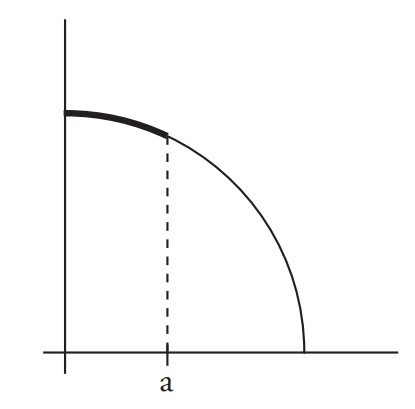
\includegraphics[width=0.3\textwidth]{arc length.jpg}
    \end{center}
    $y= \sqrt{1-x^2}$ describes the upper half of a circle with radius 1. We use \alpha to denote the arc length along the circle.
    \begin{align*}
        y' &= \frac{-x}{\sqrt{1-x^2}} \\
        ds &= \sqrt{1 + \frac{x^2}{1-x^2}}dx \\
        \alpha &= \int_{0}^{a} \frac{dx}{\sqrt{1-x^2}} \\
        &= \sin^{-1} x \Big|_{0}^{a} \\
        (sin \alpha &= a)
    \end{align*}
\end{example}

\subsubsection*{Introduction to Surface Area}
\begin{example}
    \textbf{Surface Area of a Parabola} \\
    \begin{center}
        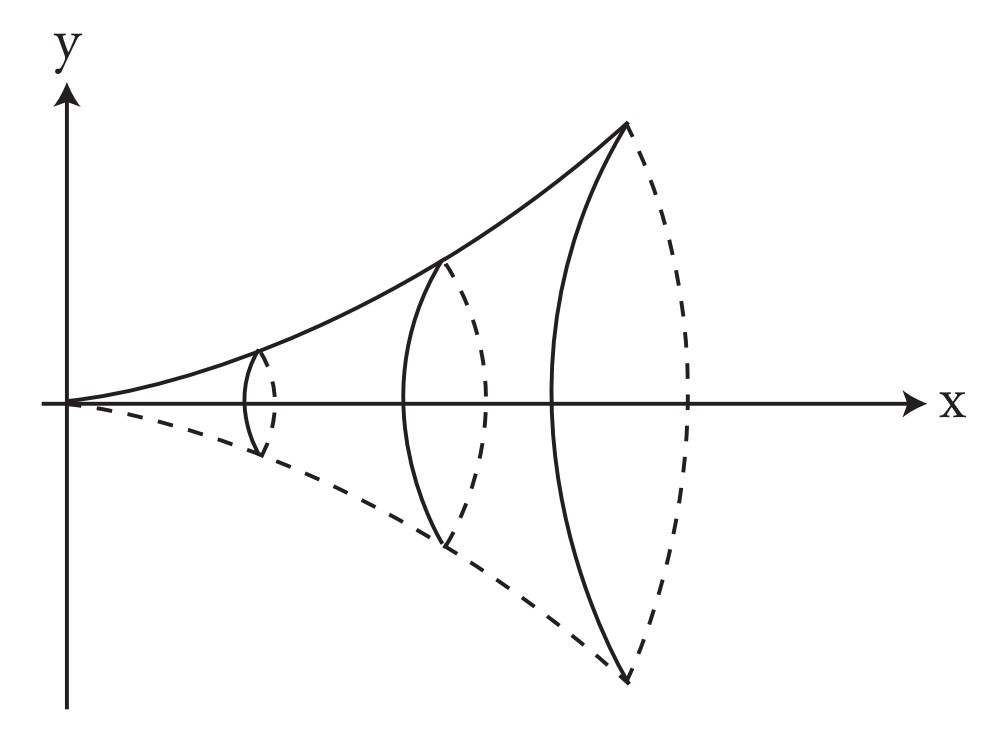
\includegraphics[width=0.3\textwidth]{parabola rotation.jpg}
    \end{center}
    \begin{align*}
        S &= \int_{0}^{a} 2 \pi y ds \\
        &= 2 \pi \int_{0}^{a} y \sqrt{1 + (y')^2} dx \\
        &= 2 \pi \int_{0}^{a} x^2 \sqrt{1 + (2x)^2} dx \\
    \end{align*}
\end{example}



\subsection{Parametric Equations and Polar Coordinates}




















\end{document}
